\documentclass{article}

\usepackage[utf8]{inputenc}
\usepackage{amsmath}
\usepackage{physics}
\usepackage{graphicx}
\usepackage[labelfont=bf]{caption}

\begin{document}
    \begin{figure}[h!]
        \centering
        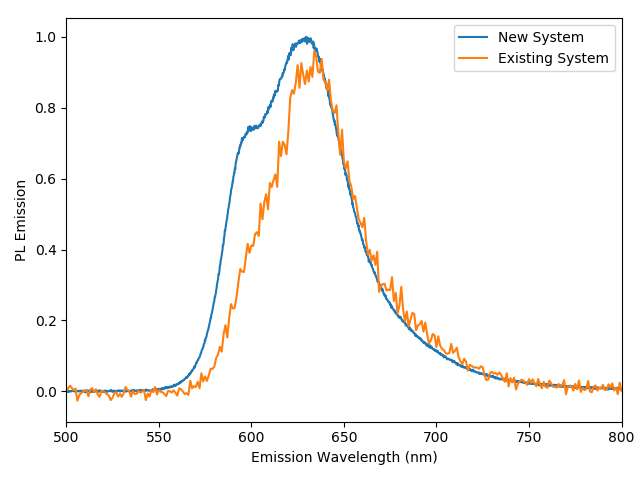
\includegraphics[width=\textwidth]{fig.png}
        \caption{Emission spectrum of ADT-TES-F, excited at 405nm. Wide-field illumination used by the existing system to excite the sample yields a noisy spectrum, and does not excite the secondary peak that is shown clearly in the results from the new system. This may be because the wide-field illumination is exciting many adjacent crystals in the sample, which emit slightly different spectra. The laser illumination in the new system has the spatial resolution necessary to illuminate single crystals.}
    \end{figure}
\end{document}